\documentclass[conference]{IEEEtran}
\usepackage[utf8]{inputenc}
\usepackage[spanish]{babel}
\usepackage{graphicx}
\usepackage{cite}
\usepackage{amsmath,amssymb,amsfonts}

\usepackage{textcomp}
\usepackage{xcolor}
\usepackage{listings}
\usepackage{booktabs}
\usepackage{lmodern}
\usepackage{microtype}
\usepackage[hyphens]{url}
\usepackage[hidelinks]{hyperref}
\setlength{\emergencystretch}{3em}

\begin{document}

\title{Bases de Datos Documentales}

\author{\IEEEauthorblockN{Juan P. Márquez Ablan}
\IEEEauthorblockA{\textit{Universidad Católica Andrés Bello}\\
\textit{jpmarquez.23@est.ucab.edu.ve}}}

\maketitle

\begin{abstract}
Las bases de datos documentales constituyen una subcategoría del paradigma NoSQL (Not Only SQL) diseñada para gestionar información no estructurada o semi-estructurada mediante unidades autónomas denominadas documentos. El presente trabajo analiza sus fundamentos teóricos, metodológicos e históricos, describe el modelo de datos adoptado para un caso de uso concreto —un marketplace de artesanías amazónicas con requisitos de localización multilingüe y procesamiento geoespacial— y evalúa su posicionamiento frente al estado del arte actual, incluyendo su papel emergente como infraestructura de soporte para sistemas de inteligencia artificial generativa.
\end{abstract}

\begin{IEEEkeywords}
bases de datos documentales, NoSQL, MongoDB, BSON, JSON, escalabilidad horizontal, GeoJSON, Big Data, inteligencia artificial.
\end{IEEEkeywords}

\section{Introducción}

Las bases de datos documentales nacieron para resolver un problema concreto: almacenar información que no encaja en una tabla clásica con filas y columnas perfectamente definidas. Imagínese un producto artesanal que tiene nombre en tres idiomas, una historia cultural asociada, fotografías, dimensiones y reseñas de clientes —todo junto, en un solo ``paquete''. Los sistemas relacionales convencionales imponen esquemas rígidos que dificultan este tipo de representación compuesta; en cambio, las bases de datos documentales permiten que cada registro defina su propia estructura según lo requiera.

Para establecer el marco de referencia del sistema de almacenamiento, la Fig.\ \ref{fig:mapaconceptual} ilustra un mapa conceptual que sintetiza la arquitectura de las bases de datos documentales. El esquema desglosa el paradigma en cuatro ejes fundamentales: (1) los \textbf{fundamentos conceptuales}, que destacan la escalabilidad horizontal y la flexibilidad dinámica del modelo; (2) los \textbf{fundamentos teóricos}, basados en la agrupación lógica mediante colecciones y estructuras de pares clave-valor; (3) las \textbf{operaciones básicas} de manipulación transaccional (CRUD: Create, Read, Update, Delete); y (4) las \textbf{herramientas tecnológicas}, resaltando motores líderes como MongoDB y los formatos de intercambio JSON/BSON. En conjunto, este diagrama evidencia cómo la unidad de agregación del documento elimina la rigidez de los esquemas relacionales, permitiendo un modelado ágil.

\begin{figure}[htbp]
\centerline{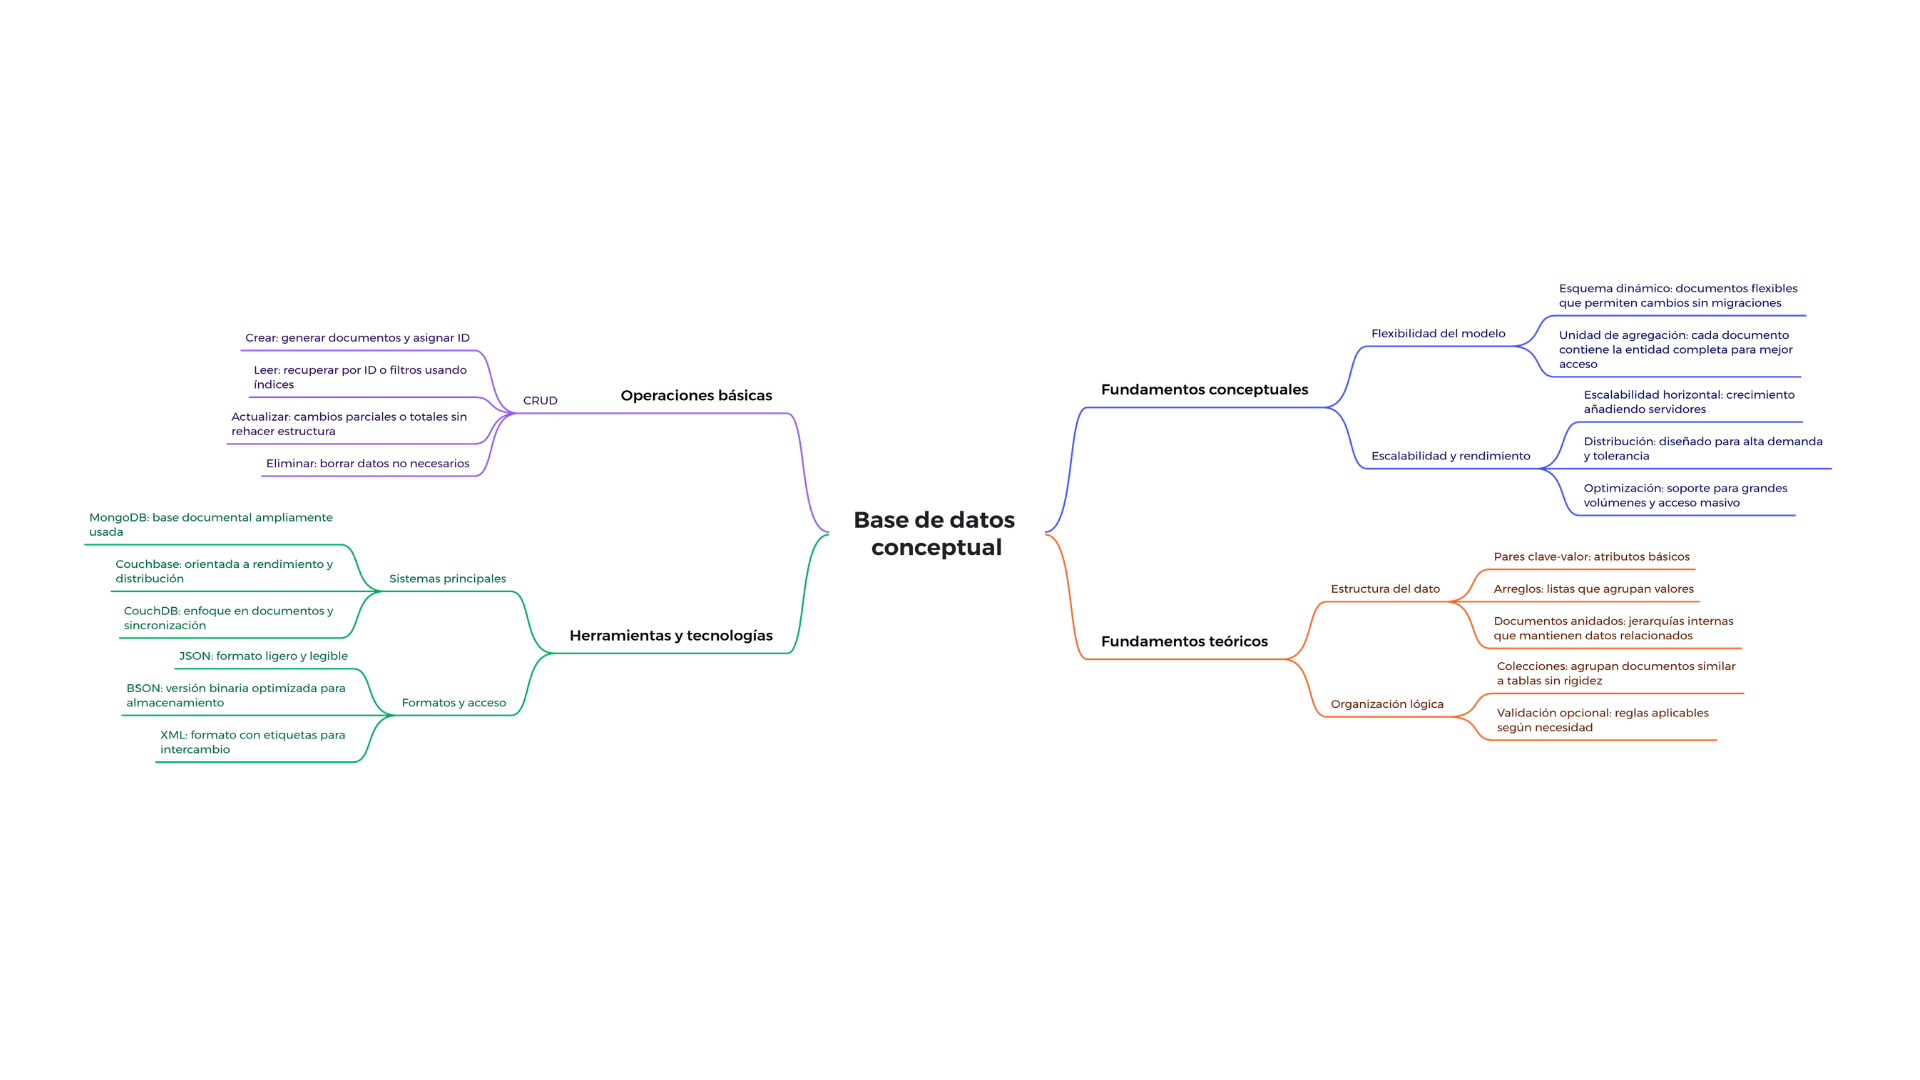
\includegraphics[width=\columnwidth]{../../Img/MapaConceptual.png}}
\caption{Mapa conceptual del ecosistema de bases de datos documentales. Se detallan los principios de flexibilidad estructural, operaciones transaccionales (CRUD) y las tecnologías de estandarización empleadas para el manejo de datos no relacionales.}
\label{fig:mapaconceptual}
\end{figure}

\section{Fundamentos Teóricos}

\subsection{Definición}
Una base de datos documental es un sistema que organiza la información en \textbf{documentos}: registros independientes y autodescriptivos que pueden tener estructuras diferentes entre sí. La analogía más intuitiva es la de una carpeta física: así como cada sobre dentro de una carpeta puede contener documentos de distinto formato y extensión, cada registro en esta base de datos puede tener sus propios campos sin seguir un molde obligatorio. A diferencia de una base de datos relacional donde todo debe seguir un esquema rígido de tablas aquí \textbf{cada documento puede tener sus propios campos y atributos}. Según Carvalho, Sá y Bernardino \cite{carvalho2023}, estos sistemas pueden manejar datos no estructurados, semi-estructurados y estructurados.

\subsection{Características Principales}
\begin{itemize}
    \item \textbf{Esquema dinámico (flexible):} no existe una estructura fija obligatoria. Cada documento puede evolucionar independientemente, lo que permite a los desarrolladores agregar o modificar campos sin procesos de migración complejos que impliquen detener el sistema.
    \item \textbf{Documentos como unidades independientes:} toda la información de una entidad vive junta en un solo registro. Esto evita la necesidad de operaciones JOIN (consultas que combinan varias tablas), que son costosas en tiempo cuando los datos crecen.
    \item \textbf{Escalabilidad horizontal:} diseñadas para crecer distribuyendo la carga en múltiples servidores mediante un mecanismo denominado sharding (particionamiento), en lugar de depender de una sola máquina cada vez más potente. Es como repartir el trabajo entre varios empleados en lugar de contratar a uno más veloz.
    \item \textbf{Alto rendimiento:} al tratar cada documento como una unidad independiente, las lecturas y escrituras son muy eficientes, incluso con grandes volúmenes de datos.
\end{itemize}

\subsection{Posicionamiento en el Ecosistema NoSQL}
Las bases de datos documentales son una \textbf{subcategoría de los sistemas NoSQL} (Not Only SQL), una familia de motores de almacenamiento que surgió como alternativa a las bases relacionales para escenarios donde la flexibilidad y la escala masiva son prioritarias. Mientras que las bases relacionales dependen de las propiedades \textbf{ACID} (Atomicidad, Consistencia, Aislamiento y Durabilidad —garantías que aseguran que cada operación se complete correctamente o no tenga efecto alguno—), los modelos documentales operan bajo el \textbf{teorema CAP} y las propiedades \textbf{BASE} (Disponibilidad Básica, Estado Flexible, Consistencia Eventual). En términos simples: priorizan que el sistema siempre esté disponible y que los datos se sincronicen entre servidores en algún momento, aunque no necesariamente de forma instantánea.

\section{Fundamentos Metodológicos}

\subsection{Formatos de Almacenamiento}
Los documentos se codifican típicamente en formatos estandarizados que permiten representar información de manera estructurada y portátil. Los más utilizados son \textbf{JSON} (JavaScript Object Notation: un formato de texto legible para humanos que organiza datos mediante pares de clave y valor), \textbf{BSON} (la versión binaria de JSON utilizada internamente por MongoDB, que agrega soporte para tipos de datos adicionales como fechas y datos binarios) y \textbf{XML} (eXtensible Markup Language: un formato más antiguo basado en etiquetas, similar al lenguaje HTML de las páginas web). JSON es el más popular por su legibilidad y compatibilidad universal.

\subsection{Conceptos Clave del Modelo}
\begin{itemize}
    \item \textbf{Pares clave-valor:} la unidad mínima de información en un documento. Funciona como un diccionario: una ``clave'' (el nombre del atributo) apunta a un ``valor'' (el dato). Por ejemplo: \texttt{"nombre": "Bolso tejido"}.
    \item \textbf{Arreglos (arrays):} listas que agrupan múltiples valores bajo una misma clave, de manera similar a una columna con varias entradas. Por ejemplo: \texttt{"etiquetas": ["ancestral", "natural", "tejido"]}.
    \item \textbf{Documentos anidados:} estructuras complejas dentro del documento principal que permiten agrupar jerárquicamente información relacionada. Es equivalente a tener una ficha técnica dentro de una ficha de producto, todo en un solo registro.
    \item \textbf{Colecciones:} agrupaciones lógicas de documentos que comparten un propósito similar (análogas a las tablas en bases relacionales, pero sin esquema fijo). Por ejemplo: una colección de ``usuarios'' y otra de ``pedidos''.
    \item \textbf{Validación de esquemas:} mecanismos opcionales que permiten imponer reglas de estructura cuando la consistencia de los datos es requerida. Funcionan como un filtro de calidad que rechaza documentos que no cumplan ciertos requisitos mínimos.
\end{itemize}

\subsection{Operaciones Básicas — CRUD}
Las cuatro operaciones fundamentales para interactuar con una base de datos documental reciben el nombre colectivo de CRUD, acrónimo de sus siglas en inglés:
\begin{itemize}
    \item \textbf{Crear (Create):} se genera un nuevo documento con un identificador único asignado automáticamente por el motor.
    \item \textbf{Leer (Read):} se consultan documentos por su identificador o por valores de sus campos. Se pueden agregar índices —estructuras internas que actúan como el índice de un libro— para acelerar las búsquedas.
    \item \textbf{Actualizar (Update):} se modifican documentos existentes, ya sea en su totalidad o parcialmente, sin necesidad de reescribir el registro completo.
    \item \textbf{Eliminar (Delete):} se remueven documentos de forma permanente de la colección.
\end{itemize}

\subsection{Herramientas Tecnológicas Principales}
\begin{itemize}
    \item \textbf{MongoDB —} la más popular a nivel mundial; usa formato BSON/JSON y es el motor de referencia de este trabajo.
    \item \textbf{CouchDB (Apache) —} pionera en bases documentales orientadas a la web; destaca por su sincronización offline.
    \item \textbf{Couchbase —} combina características de caché (almacenamiento temporal de alta velocidad) y base documental.
    \item \textbf{Amazon DocumentDB / Azure Cosmos DB —} soluciones administradas en la nube; el proveedor se encarga del mantenimiento de la infraestructura.
\end{itemize}

\section{Estado del Arte}

\subsection{Antecedentes — Línea de Tiempo}
La evolución de las bases de datos documentales puede rastrearse cronológicamente a partir de la obra de Meier y Kaufmann \cite{meier2019}:
\begin{itemize}
    \item \textbf{1989 — Lotus Notes:} aunque el término ``base de datos documental'' aún no existía, Lotus Notes introdujo un sistema colaborativo basado en documentos no tabulares en entornos empresariales, anticipando el paradigma.
    \item \textbf{1998 — Acuñación del término NoSQL:} el término fue empleado por primera vez para una base de datos que, aunque relacional, carecía de interfaz SQL \cite{meier2019}. Posteriormente se consolidó como el paraguas clasificador de las bases documentales.
    \item \textbf{Finales de los 1990 — Auge de XML:} con el estándar XML del W3C surgieron las ``bases de datos nativas XML'', predecesoras directas de los almacenes documentales actuales \cite{meier2019}.
    \item \textbf{2005 — Apache CouchDB:} sentó las bases del paradigma moderno de bases documentales orientadas a la web \cite{meier2019}. Su diseño eliminó de raíz las vulnerabilidades por inyección SQL al prescindir de ese lenguaje.
    \item \textbf{2007-2009 — MongoDB:} masificó el uso de JSON por encima de XML, estableciendo la estructura de lista de pares atributo-valor como el estándar del ecosistema \cite{meier2019}.
    \item \textbf{2010-Actualidad — Consolidación en la nube y Big Data:} las bases documentales alcanzaron la madurez para operar de manera distribuida, con soluciones administradas como Amazon DocumentDB y Azure Cosmos DB que eliminan la necesidad de gestionar servidores propios.
\end{itemize}

\subsection{Evolución Reciente — Interoperabilidad y Código Abierto}
La adopción masiva de modelos \textbf{DBaaS} (Database as a Service: bases de datos gestionadas íntegramente por un proveedor en la nube) trajo desafíos de portabilidad entre plataformas. Para mitigar esto, la comunidad de código abierto impulsó innovaciones como \textbf{DocumentDB}, donada por Microsoft a la Linux Foundation bajo licencia MIT, que integra las capacidades de MongoDB con la solidez relacional de PostgreSQL mediante una extensión nativa \cite{harper2025}.

\subsection{Perspectivas Futuras — IA y Big Data}
Las bases de datos documentales se han convertido en el pilar de soporte para ecosistemas de inteligencia artificial y modelos generativos:
\begin{itemize}
    \item \textbf{Memorias centralizadas para agentes inteligentes:} almacenan historiales de sesión, registros conversacionales de chatbots y cachés semánticas, permitiendo que los asistentes recuerden el contexto de interacciones previas.
    \item \textbf{RAG (Retrieval-Augmented Generation — Generación Aumentada por Recuperación):} los almacenes de documentos actúan como capa de caché semántica que preserva el significado subyacente de consultas, facilitando respuestas más precisas en modelos de lenguaje.
    \item \textbf{Rendimiento superior:} sus métricas en tiempos de respuesta aseguran que sigan liderando el manejo del conocimiento en bruto y la aceleración de herramientas analíticas.
\end{itemize}

\section{Casos de Uso}

\subsection{Big Data y Desarrollo Web Ágil}
El diseño de las bases documentales es ideal para el \textbf{procesamiento de Big Data} (conjuntos de datos de volumen, velocidad y variedad tan elevados que los sistemas tradicionales no pueden procesarlos eficientemente), superando las limitaciones de escalabilidad de los sistemas relacionales. Su flexibilidad es perfecta para el \textbf{desarrollo ágil}, donde los requisitos cambian constantemente y los equipos necesitan modificar la estructura de los datos sobre la marcha sin interrumpir el servicio \cite{carvalho2023}.

\subsection{IoT y Procesamiento Geoespacial}
La distribución eficiente de carga convierte a las bases documentales en infraestructura indispensable para:
\begin{itemize}
    \item \textbf{Internet de las Cosas (IoT):} gestión de redes de sensores a gran escala, donde miles de dispositivos envían datos simultáneamente y cada uno puede reportar atributos distintos.
    \item \textbf{Sistemas de Información Geográfica (GIS):} soporte nativo para el formato GeoJSON (un estándar para representar coordenadas y formas geográficas) e índices espaciales para cálculos de distancia, proximidad e intersecciones entre puntos en el mapa.
\end{itemize}

\subsection{Inteligencia Artificial y Modelos Generativos}
Soluciones como DocumentDB se usan como \textbf{historial de sesiones centralizado}, permitiendo que los asistentes virtuales retengan el contexto de la conversación a lo largo del tiempo, ofreciendo experiencias más coherentes y personalizadas.

\subsection{El Caso del Marketplace de la Amazonía}
El proyecto denominado ``Marketplace de la Amazonía'' constituye un ejemplo representativo de aplicación documental. El desafío no es sólo gestionar un catálogo de artículos, sino soportar la vasta diversidad lingüística de las tribus indígenas de la región amazónica \cite{marquez2026}. La solución documental resulta idónea por las siguientes razones:
\begin{itemize}
    \item Permite implementar un \textbf{patrón de localización dinámica} mediante atributos JSON/BSON: las traducciones a distintos idiomas se almacenan como sub-documentos dentro del mismo artículo, eliminando la necesidad de tablas auxiliares.
    \item Se evitan costosos JOINs relacionales, ya que toda la información del producto —incluyendo sus versiones en distintas lenguas— vive en un único registro.
    \item El arquitecto debe equilibrar: indexación multilingüe rápida, evitar redundancia y mantener cada documento dentro del límite físico del motor (\textbf{16 MB por documento} en MongoDB).
\end{itemize}

\section{Modelo Conceptual, Lógico y Físico}

\subsection{Modelo Conceptual}
El modelo conceptual describe las entidades principales del sistema y sus relaciones, independientemente de cómo se implementen técnicamente. Para el Marketplace de la Amazonía, las entidades identificadas son:
\begin{itemize}
    \item \textbf{Artículos:} productos artesanales con información multilingüe.
    \item \textbf{Usuarios:} clientes y vendedores de la plataforma.
    \item \textbf{Pedidos:} transacciones con detalle de artículos comprados.
    \item \textbf{Categorías:} clasificación jerárquica de productos, también localizada.
    \item \textbf{Comunidades:} tribus y comunidades indígenas con ubicación geográfica.
    \item \textbf{Reseñas:} opiniones y calificaciones de los compradores.
\end{itemize}

La Fig.\ \ref{fig:modeloconceptual} presenta el diagrama del modelo conceptual del sistema. Su diseño fue elaborado siguiendo metodologías estándar de modelado de datos para representar visualmente las relaciones y cardinalidades de alto nivel, sirviendo como mapa de ruta previo a la transcripción en colecciones NoSQL.

\begin{figure}[htbp]
\centerline{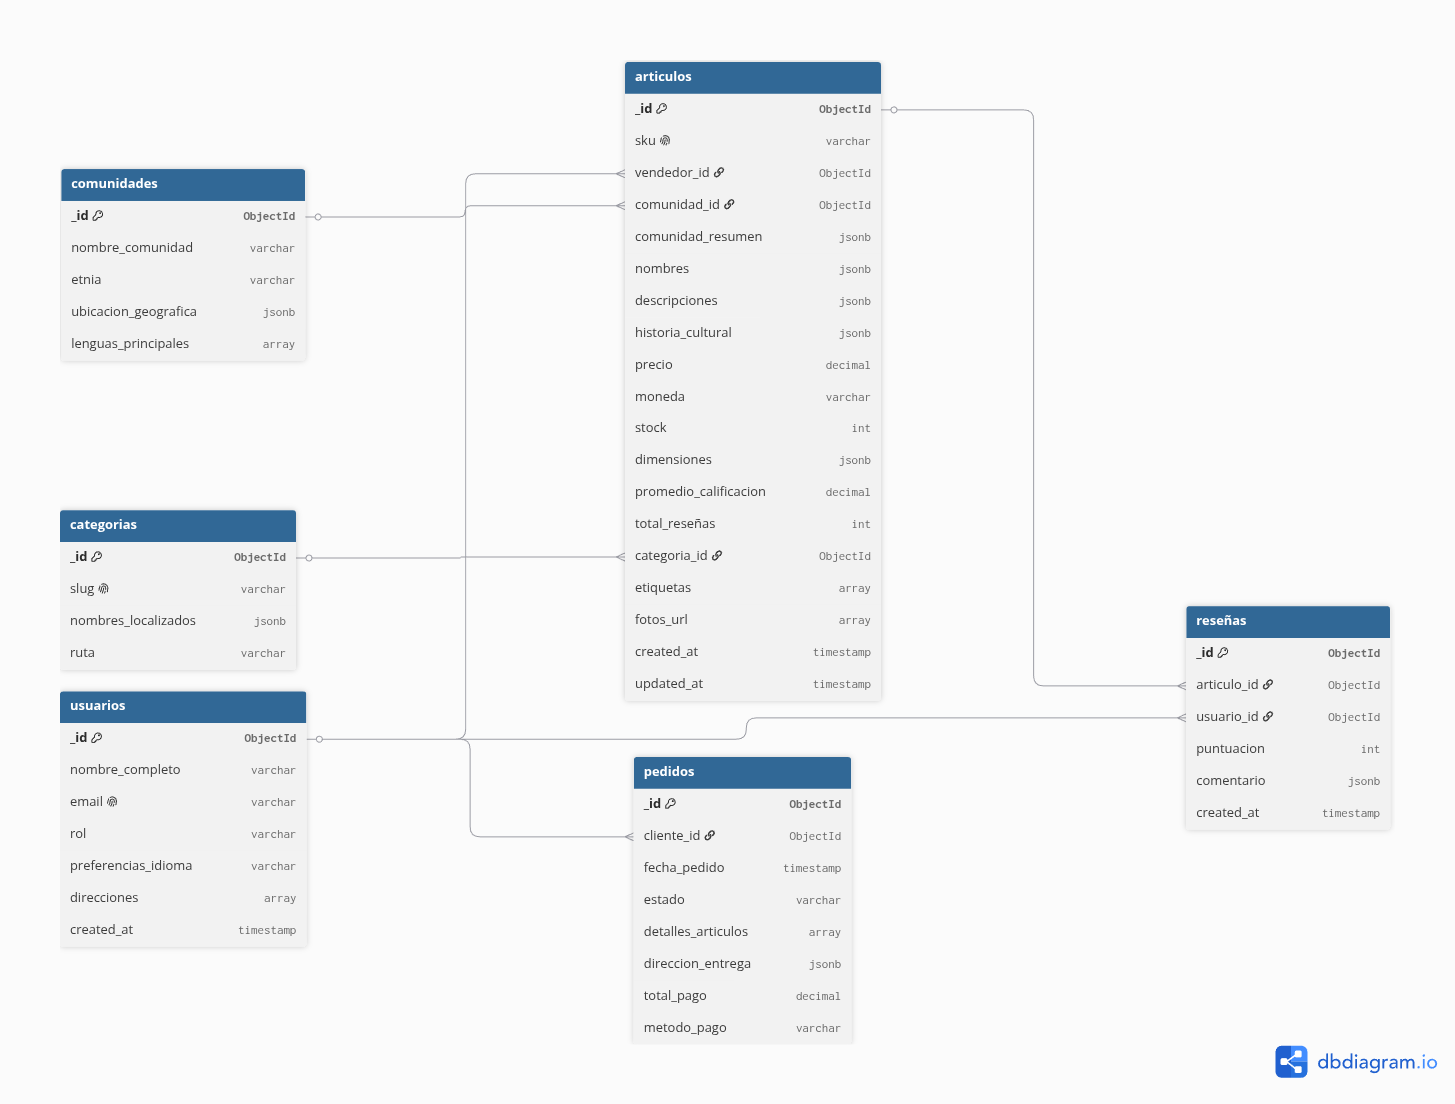
\includegraphics[width=\columnwidth]{../../Img/ModeloConceptual.png}}
\caption{Modelo conceptual del Marketplace de la Amazonía. Se representan las entidades principales (Artículos, Usuarios, Pedidos, Comunidades, Categorías y Reseñas) junto con sus relaciones y cardinalidades.}
\label{fig:modeloconceptual}
\end{figure}

\subsection{Modelo Lógico}
A diferencia de los modelos relacionales tradicionales —que expresan su diseño en tablas con columnas fijas—, el esquema lógico de esta solución se estructura mediante \textbf{colecciones de documentos BSON}, lo que permite manejar la variabilidad de atributos sin migraciones complejas. La \textbf{Tabla \ref{tab:colecciones}} resume las colecciones principales que componen el núcleo del sistema y su propósito.

\begin{table*}[htbp]
\caption{Resumen de Colecciones del Modelo Lógico}
\begin{center}
\footnotesize
\begin{tabular}{|l|p{0.3\linewidth}|p{0.45\linewidth}|}
\hline
\textbf{Colección} & \textbf{Campos Clave} & \textbf{Propósito en el Sistema} \\
\hline
\textbf{articulos} & sku, nombres (anidado), precio, comunidad\_id & Catálogo central. Almacena la data del producto y sus traducciones. \\
\hline
\textbf{usuarios} & email, rol, direcciones (arreglo) & Gestión de perfiles de clientes y artesanos/vendedores. \\
\hline
\textbf{pedidos} & cliente\_id, detalles\_articulos, estado & Trazabilidad de transacciones, montos y estatus de envío. \\
\hline
\textbf{comunidades} & nombre\_co\-mu\-ni\-dad, etnia, ubi\-ca\-cion\_geo\-gra\-fi\-ca & Registro de origen, lenguas e indexación espacial (GeoJSON). \\
\hline
\textbf{categorías} & slug, nombres\_localizados, ruta & Árbol jerárquico para la clasificación del catálogo. \\
\hline
\textbf{reseñas} & articulo\_id, puntuacion, comentario & Feedback de usuarios y consolidación de reputación. \\
\hline
\end{tabular}
\label{tab:colecciones}
\end{center}
\end{table*}

\subsection{Modelo Físico}
El modelo físico define cómo se almacenan realmente los datos en el motor de base de datos: las reglas de validación que controlan qué se puede guardar y los índices que aceleran las búsquedas. En MongoDB, esto se logra mediante dos mecanismos principales —validación de esquemas mediante \texttt{\$jsonSchema} e índices optimizados— que se detallan en los Apéndices A y B de este documento.

\section{Operaciones y Consultas al Sistema}
El diseño de la base de datos permite resolver requerimientos complejos de negocio nativos del paradigma documental, minimizando la carga de procesamiento en el lado de la aplicación (backend). Entre las operaciones principales soportadas se encuentran:
\begin{itemize}
\begin{sloppypar}
    \item \textbf{Búsquedas de texto completo (Full-Text Search):} el motor analiza lingüísticamente el texto de los campos configurados y devuelve resultados ordenados por relevancia, de manera similar a como funciona un buscador web. Se implementan mediante índices de texto sobre los atributos de nombres y descripciones.
\end{sloppypar}
    \item \textbf{Filtros jerárquicos y ordenamiento:} extracción de catálogos indexados por categorías y ordenados por precio o calificación, permitiendo navegar el inventario de forma eficiente.
    \item \textbf{Análisis espacial (GIS):} dada la dispersión geográfica de las comunidades indígenas, el modelo explota el estándar GeoJSON y los operadores geoespaciales nativos del motor para calcular distancias y encontrar comunidades cercanas a un punto dado.
\end{itemize}

A modo de ilustración, el \textbf{Listado 1} muestra una consulta geoespacial concreta: dadas unas coordenadas de latitud y longitud, el sistema devuelve todas las comunidades indígenas ubicadas dentro de un radio de 50 km, aprovechando los índices espaciales del motor sin necesidad de cálculos manuales de distancia.

\begin{lstlisting}[caption={Consulta geoespacial para localización de comunidades en un radio de 50 km.}, label={lst:geo}, breaklines=true, basicstyle=\footnotesize\ttfamily]
db.comunidades.find({
  "ubicacion_geografica.coordenadas": {
    $near: {
      $geometry: {
        type: "Point",
        coordinates: [-70.00, -3.80]   // longitud, latitud
      },
      $maxDistance: 50000              // radio en metros (50 km)
    }
  }
});
\end{lstlisting}

El abanico completo de consultas operativas —incluyendo proyecciones, agregaciones complejas y búsquedas transaccionales básicas— se encuentra documentado en el repositorio de código complementario asociado a este trabajo \cite{marquez2026}.

\section{Conclusiones y Recomendaciones}

\subsection{Características Clave}
\begin{itemize}
    \item \textbf{Esquema flexible:} permiten evolucionar la estructura de los datos sin migraciones costosas.
    \item \textbf{Alto rendimiento en lectura y escritura:} ideales para aplicaciones con grandes volúmenes de datos.
    \item \textbf{Escalabilidad horizontal nativa:} crecen distribuyendo datos en múltiples nodos mediante sharding.
    \item \textbf{Formatos legibles:} JSON/BSON son intuitivos tanto para humanos como para máquinas.
    \item \textbf{Soporte geoespacial:} índices espaciales nativos para aplicaciones GIS e IoT.
    \item \textbf{Ecosistema maduro:} herramientas robustas como MongoDB, CouchDB y soluciones en la nube.
\end{itemize}

\subsection{¿Cuándo Emplear una Base de Datos Documental?}
\begin{itemize}
    \item Cuando los datos tienen \textbf{estructura variable o semi-estructurada}.
    \item Cuando se necesita \textbf{desarrollo ágil} con cambios frecuentes en el esquema.
    \item En aplicaciones de \textbf{Big Data}, \textbf{IoT} o \textbf{procesamiento geoespacial}.
    \item Para \textbf{catálogos de productos} con atributos heterogéneos.
    \item En sistemas que requieren \textbf{localización multilingüe} dinámica.
    \item Como \textbf{almacén de sesiones} o \textbf{caché semántico} para aplicaciones de IA.
\end{itemize}

\subsection{¿Cuándo NO Emplearlas?}
\begin{itemize}
    \item Cuando los datos son \textbf{altamente relacionales} y requieren múltiples JOINs complejos: las bases relacionales son superiores en ese escenario.
    \item Cuando se necesitan \textbf{transacciones ACID estrictas} entre múltiples documentos o colecciones simultáneamente.
    \item Para sistemas con \textbf{esquemas muy estables} donde la rigidez relacional es una ventaja, no un obstáculo.
\end{itemize}

\subsection{Recomendaciones Finales}
\begin{itemize}
    \item \textbf{Desplazar la integridad a la aplicación:} al no haber esquemas fijos, el desarrollador debe encargarse de validar la consistencia desde la lógica de negocio. Se recomienda usar esquemas de validación (\texttt{\$jsonSchema}) siempre que sea posible.
    \item \textbf{Diseñar orientado a las consultas:} la estructura del documento debe optimizarse para las lecturas más frecuentes, no para evitar redundancia como en el modelo relacional.
    \item \textbf{Monitorear el tamaño de los documentos:} en MongoDB el límite es de 16 MB por documento. Es importante planificar el modelo para no excederlo.
    \item \textbf{Implementar una estrategia de índices equilibrada:} los índices aceleran dramáticamente las consultas, pero un exceso de ellos ralentiza las escrituras. Debe encontrarse el balance adecuado.
    \item \textbf{Considerar la seguridad desde el inicio:} en entornos DBaaS, establecer protocolos de cifrado robustos para datos sensibles \cite{khan2023}.
\end{itemize}



\appendices
\section{Validación Estricta de Esquemas (\texttt{\$jsonSchema})}
El mecanismo \texttt{\$jsonSchema} funciona como un contrato que el motor evalúa antes de aceptar cualquier inserción o modificación: si un documento no cumple las reglas definidas, la operación es rechazada. A continuación se describen las reglas implementadas sobre la colección de \textit{pedidos}, que es la colección más crítica del sistema por involucrar transacciones económicas:
\begin{itemize}
    \item \textbf{Integridad referencial:} el campo \textit{cliente\_id} exige estrictamente el tipo de dato ObjectId (el identificador interno de MongoDB), evitando que se registren pedidos con referencias a usuarios inexistentes o con formatos incorrectos.
    \item \textbf{Restricciones de dominio:} el campo \textit{estado} está restringido a una enumeración finita (\textit{enum}) de valores predefinidos —tales como \textit{pendiente}, \textit{enviado} o \textit{entregado}— garantizando que el sistema nunca contenga estados inválidos que rompan la lógica del negocio.
    \item \textbf{Validaciones numéricas y de cardinalidad:} se imponen límites inferiores automáticos (montos de pago mayores o iguales a cero) y se garantiza que el arreglo de detalles de artículos contenga al menos un elemento (\textit{minItems: 1}), impidiendo pedidos vacíos.
\end{itemize}

\section{Estrategia de Indexación}
Un índice en una base de datos funciona de manera análoga al índice de un libro: en lugar de leer cada página para encontrar un tema, se consulta el índice para ir directamente a la página correcta. Para mitigar la latencia en un catálogo con potencial de escalado, se diseñó una arquitectura de índices en tres niveles sobre la colección de \textit{articulos}:
\begin{itemize}
    \item \textbf{Índices Únicos:} aplicados a claves de negocio como \textit{sku} (el código de identificación único de cada producto), para prevenir duplicados a nivel físico.
    \item \textbf{Índices Compuestos:} combinan dos o más campos en un único índice orientado a optimizar las consultas más frecuentes de la interfaz. Por ejemplo, un índice sobre \textit{categoria\_id} y \textit{precio} evita que el motor tenga que revisar toda la colección (\textit{collection scan}) para devolver el catálogo filtrado y ordenado.
    \item \textbf{Índices de Texto (Full-Text Search):} permiten búsquedas semánticas sobre los atributos de internacionalización. Se asignaron pesos ponderados (10 para \textit{nombres.es} frente a 5 para \textit{descripciones.es}) para que el algoritmo de relevancia priorice coincidencias en el título del producto sobre el texto de su descripción.
\end{itemize}
\begin{thebibliography}{00}
\hbadness=10000
\bibitem{carvalho2023} I. Carvalho, F. Sá, and J. Bernardino, ``Performance Evaluation of NoSQL Document Databases: Couchbase, CouchDB, and MongoDB,'' \textit{Algorithms}, vol. 16, no. 2, art. 78, 2023. doi: 10.3390/a16020078.
\bibitem{meier2019} A. Meier and M. Kaufmann, \textit{SQL \& NoSQL Databases: Models, Languages, Consistency Options and Architectures for Big Data Management}, 1st ed. Cham: Springer, 2019.
\bibitem{harper2025} J. Harper, ``What DocumentDB Means for Open Source,'' \textit{The New Stack}, Dec. 3, 2025. [En línea]. Disponible en: \url{https://thenewstack.io/what-documentdb-means-for-open-source/}
\bibitem{khan2023} W. Khan et al., ``SQL and NoSQL database software architecture performance analysis and assessments---A systematic literature review,'' \textit{Big Data and Cognitive Computing}, vol. 7, art. 97, 2023. doi: 10.3390/bdcc7020097.
\bibitem{marquez2026} J.~P. Márquez Ablan, \textit{amazonia-marketplace-db}. GitHub, 2026. [En línea]. Disponible en: \href{https://github.com/JotaPert/amazonia-marketplace-db}{\url{https://github.com/JotaPert/amazonia-marketplace-db}}
\bibitem{mongodb2026} MongoDB, ``Document Database,'' MongoDB, Inc. [En l\'{\i}nea]. Disponible en: \href{https://www.mongodb.com/es/resources/basics/databases/document-databases}{\url{https://www.mongodb.com/es/resources/basics/databases/document-databases}} [Accedido: Jun. 2026].
\end{thebibliography}

\end{document}
